According to the U.S. Energy Information Administration (EIA), global energy consumption is projected to increase by 50\% by 2050, relative to 2019, as shown in Figure \ref{fig:energyconsumption}\cite{eia_ieo2019}. This massive surge is largely driven by strong economic and population growth in non-OECD\footnote{Organisation for Economic Co-operation and Development} countries, particularly in Asia, alongside rapid urbanization and rising regional incomes. Accompanied with the ongoing shift toward electrification in end-use sectors, electricity generation is projected to increase by 79\% between 2018 and 2050, as explained in Figure \ref{fig:electricitygeneration}. Meeting this surging energy demand while simultaneously mitigating climate impact has made the transition to carbon neutrality an essential global imperative. This paradigm shift requires unprecedented cooperation across all sectors and has significantly accelerated the deployment of distributed renewable energy resources, which are projected to be the fastest-growing global energy source, alongside electrified transportation, as seen in Figure \ref{fig:renewablenergy}.
\begin{figure}
    \centering
    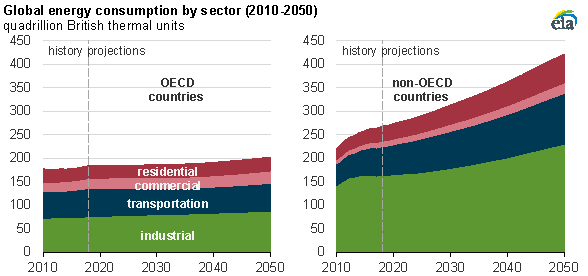
\includegraphics[width=0.9\columnwidth]{figures_intro/projection_energyuse.pdf}
    \caption{Projected increase in global energy consumption by 2050: (left) in OECD Countries, (right) in developing countries.}
    \label{fig:energyconsumption}
\end{figure}

\begin{figure}
    \centering
    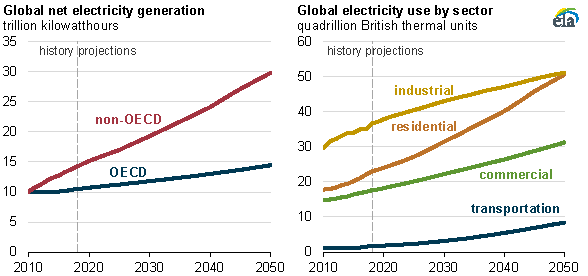
\includegraphics[width=0.9\columnwidth]{figures_intro/intro_energyuse.pdf}
    \caption{Projected increase by 2050 in electricity generation (left) and in electricity use (right) according to different sectors.}
    \label{fig:electricitygeneration}
    
\end{figure}

\begin{figure}
    \centering
    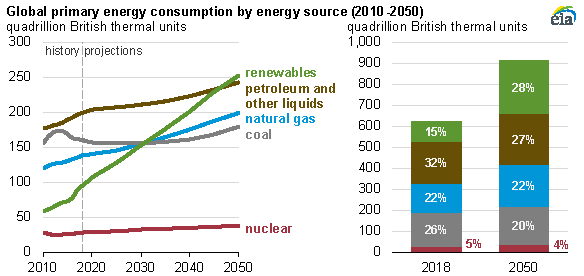
\includegraphics[width=0.9\columnwidth]{figures_intro/renewable_energy.pdf}
    \caption{Projected energy consumption by energy source by 2050.}
    \label{fig:renewablenergy}
\end{figure}
To support this massive, sustainable transition, the underlying electrical distribution infrastructure requires next-generation power conversion systems that are not only highly efficient but also exceptionally compact and reliable. Today, one of the key technologies facilitating these stringent requirements is the Solid State Transformer (SST). SSTs represent an advanced class of power electronic converters equipped with medium-frequency (MF) or high-frequency (HF) galvanic isolation, typically operating between medium-voltage (MV) distribution grids and low-voltage (LV) consumer systems. In this regard, the following sections present the characteristics, applications, and challenges associated with the development of high-power SSTs.

\section{The Solid State Transformer}
The SST is an ongoing trend today in Power Electronics. In higher power applications, to distribute power from the medium-voltage grid to an isolated low-voltage load, the traditional line frequency (50/60 Hz) transformer is commonly used, as represented in Figure \ref{fig:linefrequency}.

\begin{figure}
    \centering
    \subfloat[]{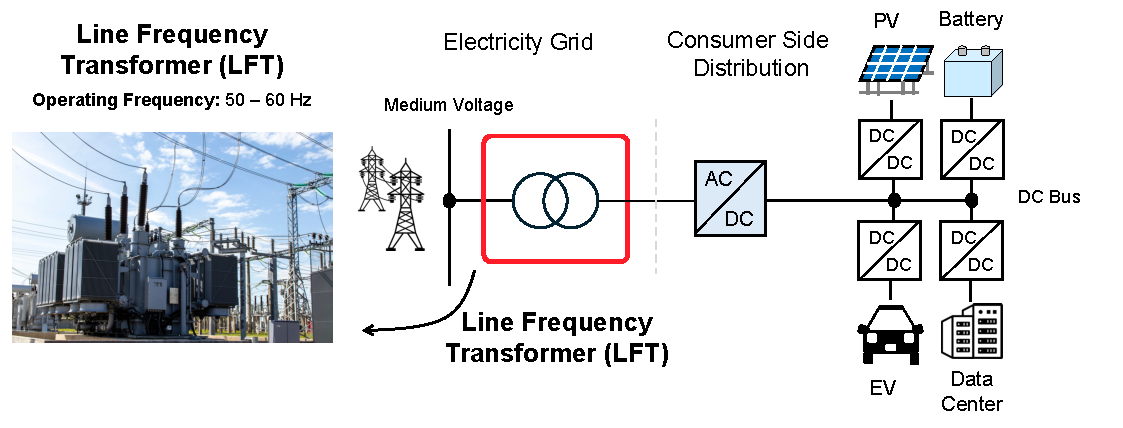
\includegraphics[width=\columnwidth]{figures_intro/linefrequency.pdf}\label{fig:linefrequency}}
\\
    \subfloat[]{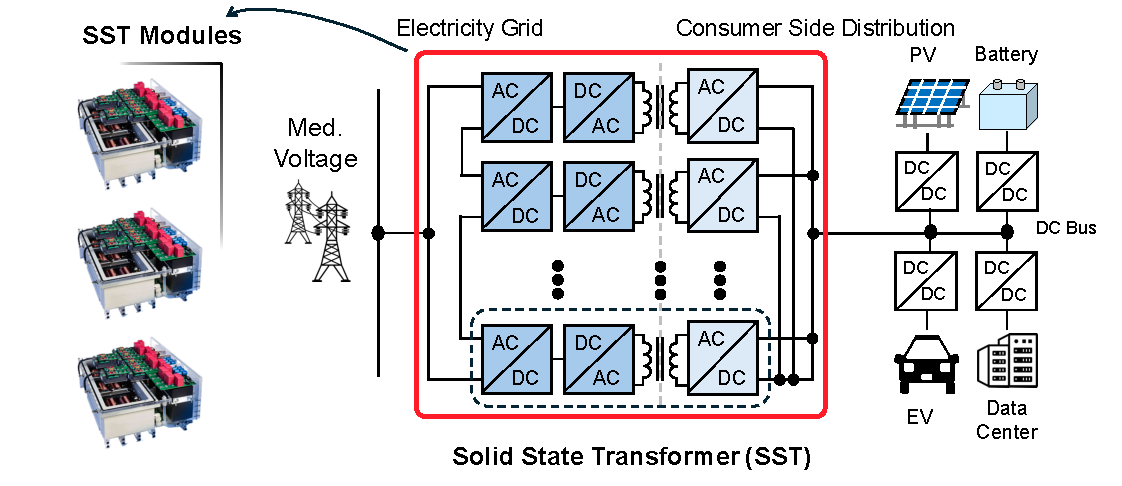
\includegraphics[width=\columnwidth]{figures_intro/SST.pdf}\label{fig:SST}}
\\
     \subfloat[]{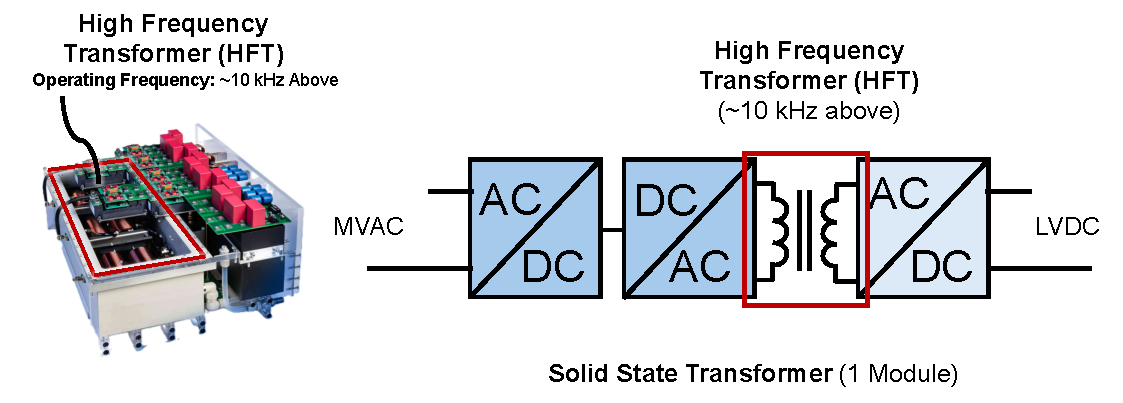
\includegraphics[width=\columnwidth]{figures_intro/module.pdf}\label{fig:module}}
    \caption{Architectures in power distribution: (a) utilizes the Line Frequency Transformer between the MV and LV stage; (b) utilizes the Solid State Transformer (SST) instead with an HFT for galvanic isolation; (c) shows one module of the SST described in (b). The HFT facilitates power transfer from the MV stage to the LV stage. SST Module is from \cite{sstexample} and is included here just for demonstration purposes. LFT is from \cite{lftexample}.}
\end{figure}

The SST is generally characterized by a multi-stage topology \cite{technologies13020074}. To overcome the spatial and weight limitations of line transformers, the SST replaces the massive 50/60 Hz core with a multi-stage architecture comprising wide-bandgap (WBG) semiconductor converters coupled with a high-frequency (HFT) (or medium-frequency (MFT)) isolation transformer. This is most commonly implemented in the isolation stage between the medium-voltage and low-voltage line. A representation of its integration in the power grid is shown in Figure \ref{fig:SST}, and a representation of one module along with the HFT in Figure \ref{fig:module}. The shown representation is just one of the many topologies and applications of the SST and is intended as a general explanatory figure. 

Instead of directly coupling the primary and secondary AC grids using a single magnetic core, the following happens through three main parts connected in series. First, the input AC power (MV) is rectified. Next, a lighter HFT/MFT provides galvanic isolation and voltage stepping. Finally, the output is converted back to DC or AC depending on the application. The mode of conversion for the isolation stage depends on the system configuration or application. To allow for the increase in power generation, as seen in Figure \ref{fig:SST}, the input side of the modules are connected in series to accommodate the MV grid, whereas the output converters are connected in parallel to accommodate higher load currents.

The benefits of SSTs mainly encompass the enabling the broad possibilities of controllability and advanced functions, including but not limited to: reactive power compensation, active filtering, fault handling, its potential for modularity, and the potential for low-voltage DC link for easy integration of various systems. As one of the main goals is to improve power density by replacing the line frequency transformer, then a lot of applications are gaining interest. These include but are not limited to high-power EV charging, future traction applications, data centers, renewable energy applications, and even smart grid systems \cite{10667423}, \cite{6342269}, \cite{8962031}, \cite{czyz2021}. 

As highlighted in recent state-of-the-art reviews of SST technologies, the viability of these systems has been greatly accelerated by the maturity of Silicon Carbide (SiC) and Gallium Nitride (GaN) devices. With semiconductor technology advancing rapidly, research has now shifted towards optimizing the power converter topologies and, most critically, improving the HFT/MFT that form the isolation stage of the SST. 

With the advent of high frequency operation, according to Faraday's Law, operating at elevated frequencies allows the magnetic core area and the number of winding turns to be drastically reduced. This results in a system that offers a fraction of the size and weight of a traditional line transformer while providing enhanced control over bidirectional power flow and fault isolation  \cite{10667423}, \cite{6342269}, \cite{8962031}, \cite{czyz2021}. 

An example is shown in Figure \ref{app:downsizing}. By the Area Product Method, scaling from 60 Hz to 10 kHz can might be able to provide about 98\% reduction in transformer volume, as shown in Figure \ref{fig:downsizing}a.  Details are shown in the Appendix: \nameref{app:downsizing}. But, as a trade-off, with more core and winding losses at higher frequency, thermal management becomes a problem for the HFT, as shown in the example provided in Figure \ref{fig:downsizing}b \cite{downsizing}. 

\begin{figure}
    \centering
    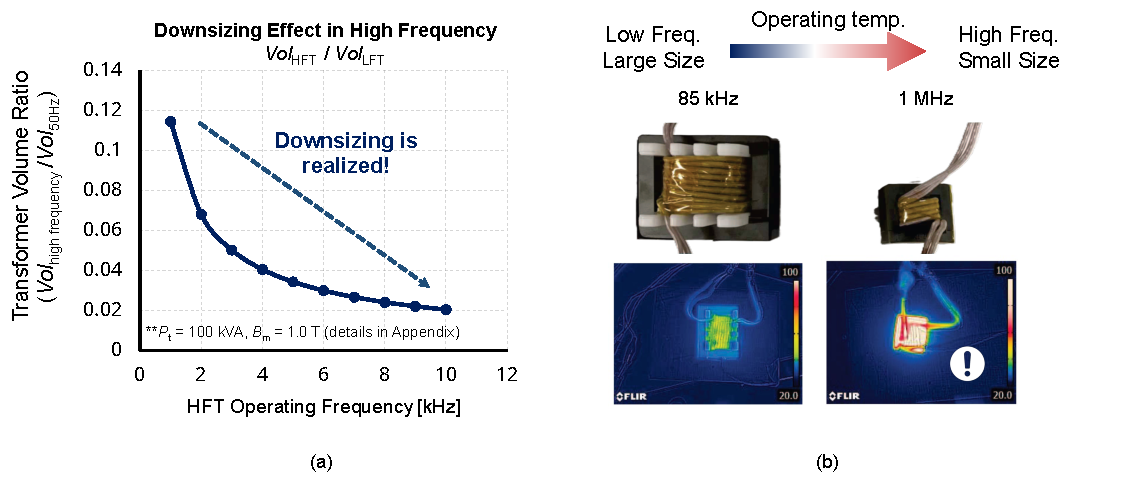
\includegraphics[width=\columnwidth]{figures_intro/downsizing.pdf}
    \caption{Operation at higher frequency brings benefits with a trade-off: (a) downsizing effect from the LFT as an effect of HF operation, details shown in Appendix \nameref{app:downsizing}; (b) thermal management trade-off shown in \cite{downsizing}.}\label{fig:downsizing}
    
\end{figure}

This profound downsizing effect renders solid-state transformers (SSTs) more essential than ever for modern power networks. Traditional line-frequency transformers (LFTs) rely on massive quantities of copper, magnetic materials, and other physical resources, consuming substantial natural resources to construct, transport, and maintain. By transitioning to a high-frequency SST architecture, this physical bulk is drastically mitigated. The resulting reduction in raw volume and weight not only alleviates the strain on global material supply chains but also significantly reduces manufacturing lead times and heavy-lift installation logistics. Furthermore, overcoming strict spatial constraints is increasingly critical for emerging applications where the highly compact footprint of a high-frequency transformer provides a decisive physical and economic advantage. However, the transition has some challenges as will be explained.
\section{Challenges in the Isolation Transformer Design} \label{sec:challenge}
The HFT/MFT in the isolation stage performs the same function as the traditional
50/60 Hz transformer which is to enable voltage transformation and provide electrical isolation between MV/HV and LV sides. However, a key feature is the operation at higher voltages and frequencies. This creates new challenges in the pillars of transformer design:
\begin{itemize}
    \item \textbf{Efficiency}: as explained in the previous section, with higher frequency and voltage operation means the increase of both core and winding losses. Primarily, for core losses, this means the selection of material that will provide high saturation flux density, compatible operating temperature, and low-loss in the desired operation condition \cite{ref1}. For winding losses, this entails careful winding methods to eliminate the effects of skin and proximity losses.
    \item \textbf{Reliability}: The transformer must simultaneously guarantee robust dielectric isolation under high-voltage stress and effectively manage skyrocketing volumetric heat to prevent thermal failure \cite{6d7bedeb4d374ffaa54effc19030ffd3, https://doi.org/10.1049/hve2.12424}.  
\end{itemize}

While dielectric isolation can be addressed by using improved dielectric material or using a thicker isolation material as well, it is important to note that this affects the thermal management performance of the transformer. Therefore, any attempt to further miniaturize the high-power isolation transformer is limited not primarily by electromagnetics, but by the physical inability to extract heat. 

\section{Thermal Management and Assembly Methods for the HFT}\label{sec:cooling}
The thermal management method for the HFT, as it is a critical part of the overall system packaging, heavily influences the final volumetric power density of the SST. To effectively manage skyrocketing volumetric heat and prevent thermal failure under high-voltage stress, various thermal management methods are currently employed in both academic research and industry.

\subsection{Active Cooling}
Active cooling encompasses the use of forced-air or liquid cooling to accelerate convective heat transfer from the transformer to the ambient environment. While highly effective at managing surface temperatures, active cooling introduces a severe penalty to the power density of the system due to the additional required custom fixtures, mounts, or other components to realize the setup. Liquid cooling systems provide superior heat transfer coefficients but require complex plumbing, pumps, and external radiators. Some examples of transformers built for these systems are shown in Figure \ref{fig:activecooling}a, \ref{fig:activecooling}b, and \ref{fig:activecooling}c \cite{leibl2017design}, \cite{chen2018high}, \cite{mogorovic2019100kw}. 

\begin{figure}[h!]
    \centering
    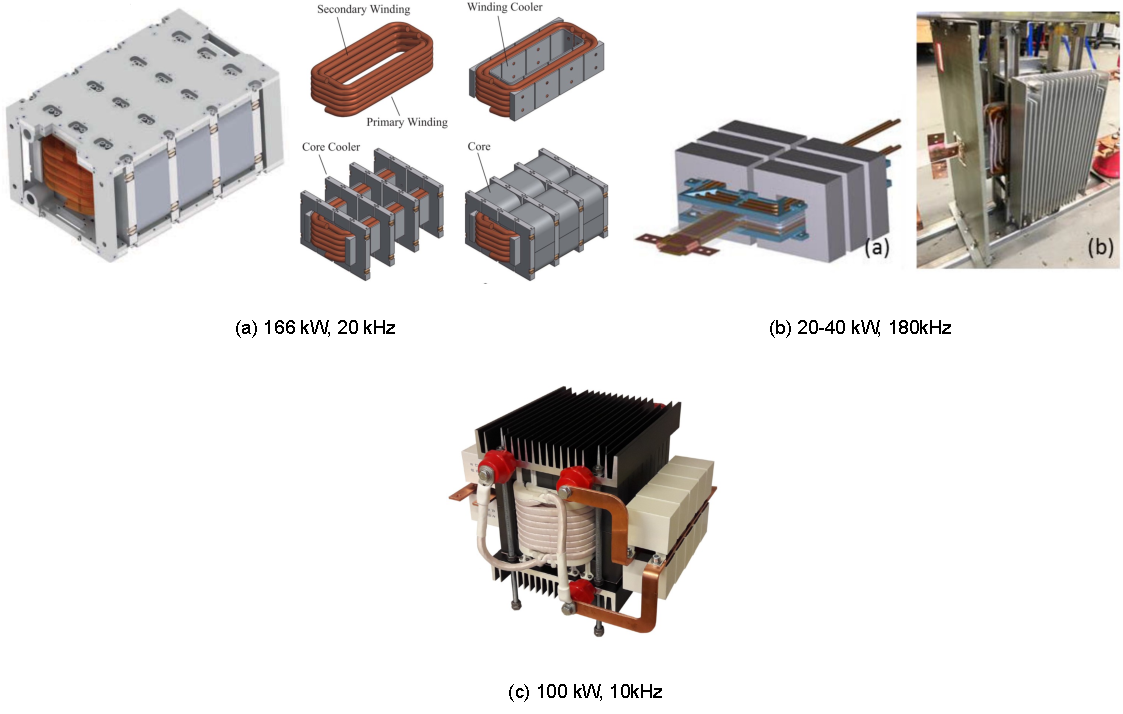
\includegraphics[width=\columnwidth]{figures_intro/forcedair_trans.pdf}
    \caption{Examples of transformers designed for active cooling. (a) is a 166 kW, 20 kHz transformer cooled using liquid cooling \cite{leibl2017design}, (b) is a 20-40 kW, 180 kHz transformer cooled using forced air cooling \cite{chen2018high}, and (c) is a 100 kW, 10 kHz transformer cooled using forced air cooling \cite{mogorovic2019100kw}.}\label{fig:activecooling}
\end{figure}

\subsection{Oil Immersion}
One of the most common methods of thermal management in the high-power domain is the use of oil immersion. While highly effective in both electrical insulation and convective heat transfer, especially when utilizing oil-directed (OD) cooling channels pumped directly through the windings, this method require heavy, bulky sealed tanks, pumps, and external heat exchangers. Furthermore, they introduce significant environmental concerns, maintenance burdens, and flammability hazards, making them undesirable for modern, compact applications \cite{6342269}. Some examples of transformers built for these systems are shown in Figure \ref{fig:oilcooling}a, and Figure \ref{fig:oilcooling}b \cite{anurag2022gen3}, \cite{cremasco2024166kw}. 

\begin{figure}[h!]
    \centering
    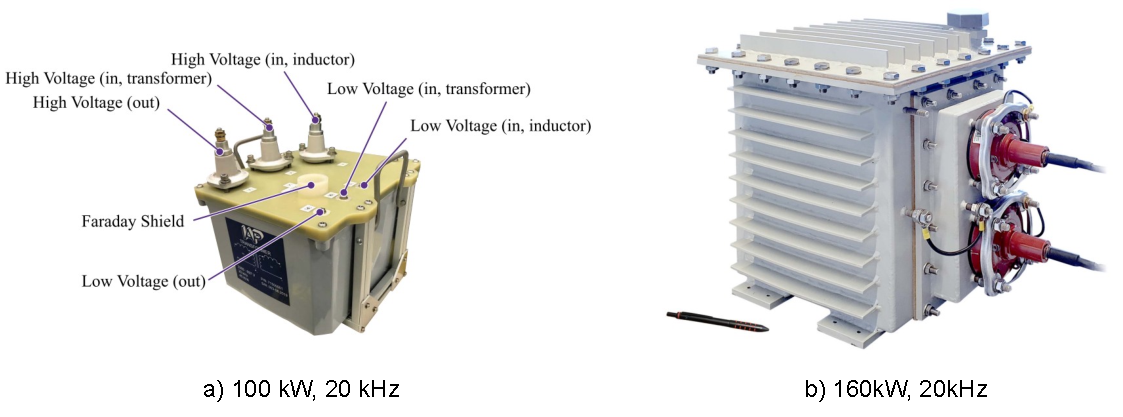
\includegraphics[width=\columnwidth]{figures_intro/oilcooled_trans.pdf}
    \caption{Examples of transformers designed for oil immersion cooling. (a) is a 100 kW, 20 kHz transformer cooled using oil immersion \cite{anurag2022gen3}, and (b) is a 160 kW, 20 kHz transformer cooled using ester oil immersion \cite{cremasco2024166kw}.}\label{fig:oilcooling}
\end{figure}

\subsection{Dry Casting}
To avoid the drawbacks of oil, dry-type medium-frequency transformers heavily rely on epoxy resin dry casting. Vacuum-cast epoxy provides exceptional, partial-discharge-free medium-voltage insulation and structural rigidity, completely encapsulating the core and windings. However, a major fundamental drawback of dry casting is thermal resistance. Standard epoxy resins possess a relatively low thermal conductivity compared to the copper windings they encase. Consequently, the potting material inherently creates a severe thermal barrier, requiring carefully designed cooling systems. Some examples of transformers utilizing this technique is shown in Figure \ref{fig:drycast}a, and \ref{fig:drycast}b \cite{yi2022design}, \cite{gradinger2017novel}. 

\begin{figure}[h!]
    \centering
    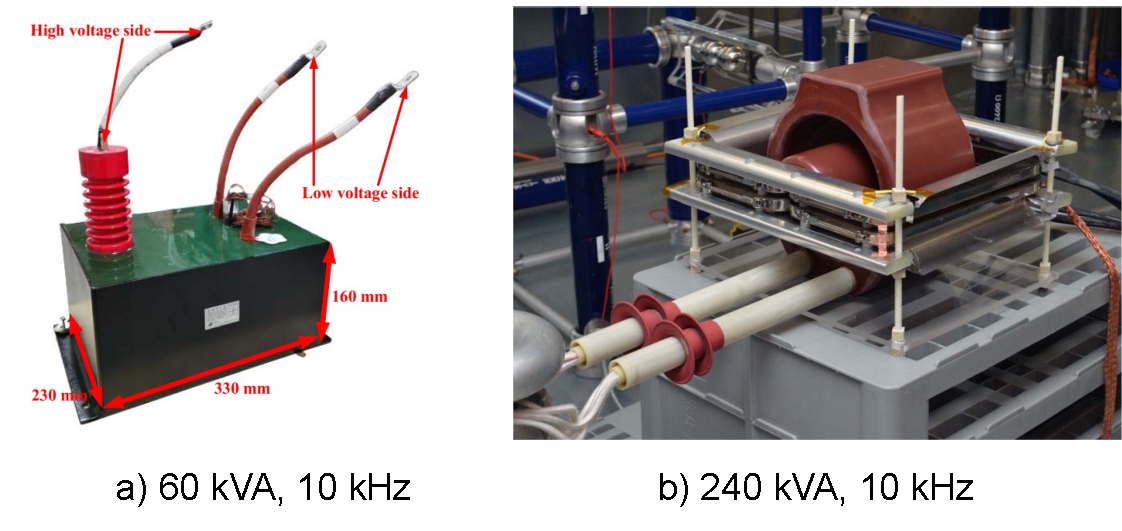
\includegraphics[width=0.7\columnwidth]{figures_intro/drycast_trans.pdf}
    \caption{Examples of transformers assembled using dry casting. (a) is a 60 kVA,10 kHz transformer \cite{yi2022design}, and (b) is a 240 kVA, 10 kHz \cite{gradinger2017novel}.}\label{fig:drycast}
\end{figure}

\subsection{Custom-designed Components}
To circumvent the limitations of standard cooling methods, some researchers utilize the design or insertion of custom components to improve the performance of active cooling or improve internal heat conduction. For instance, optimized 3D-printed bobbins to facilitate specific cooling channels, improving the overall power density by guiding air directly through the core window \cite{ref8, ref9}. Another example involves adding a metal plate in between the ferrite cores to improve heat conduction from the internal core structure into the external heat sink, bypassing the poor thermal conductivity of the ferrite material itself \cite{ref10}. Aside from being highly customized and complex to manufacture, these component-level additions primarily address core heat or surface airflow. They do not fundamentally resolve the geometric winding bottlenecks trapping heat deep within the copper layers.

\begin{figure}[h!]
    \centering
    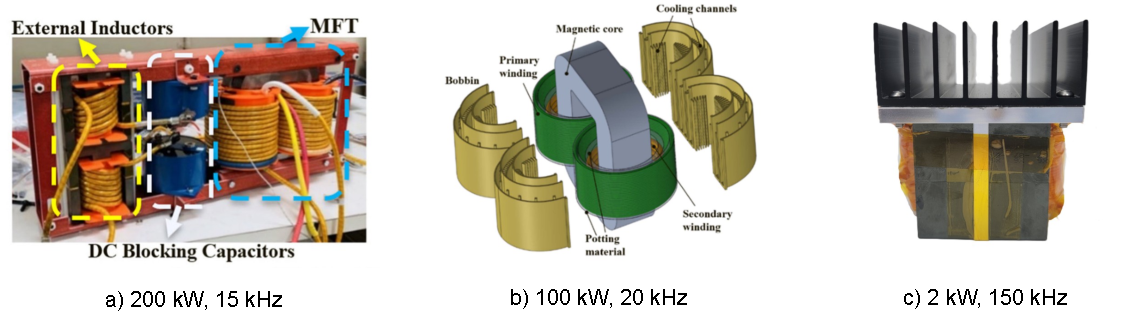
\includegraphics[width=\columnwidth]{figures_intro/custom_trans.pdf}
    \caption{Examples of transformers designed with custom components integrated, and used with other cooling systems: (a) is a 200 kW, 15 kHz transformer \cite{ref8} and (b) is a 100 kW, 20 kHz transformer that both utilize custom designed bobbins for optimized forced air cooling \cite{ref9}, and (c) is a 2 kW, 150 kHz transformer utilizing metal plates sandwiched in between cores for enhanced heat extraction \cite{ref10}.}\label{fig:customtrans}
\end{figure}

It is important to note that the design of cooling and assembly systems for transformers depend on the specific requirements and applications, thus there is no best design for the transformer. While these external and material-based thermal management methods are necessary, addressing the conflict at the foundational geometric level is a promising research direction and has not been currently examined in detail. It presents a highly promising and necessary solution for next-generation SSTs as a potential to reduce dependence on additional thermal management systems. 

\section{The Concept of a Transformer for Improved Intrinsic Thermal Management}
These transformers often use Litz wire to accommodate high current while reducing AC losses at higher frequencies. However, the poor thermal conductivity and low fill factor of Litz wire create a fundamental thermal bottleneck, hindering effective heat extraction \cite{ref11}, \cite{ref12}, which in turn forces a reliance on the aforementioned bulky and complex external cooling systems.

This work therefore investigates a contrasting design approach that prioritizes intrinsic thermal performance of the transformer. Rectangular windings are known to offer advantages like high current capacity and excellent fill factor, and they are applied as well to inductors \cite{ref22}, \cite{ref23}. However, a characterization of their thermal properties in the specific context of transformers is limited. Additionally, most of the transformers presented in the previous discussion do not use a planar structure. 

To address this, a low-profile planar structure is proposed that utilizes solid rectangular conductors arranged in a flatwise orientation, as shown in Figure \ref{fig:concept_trans}, with its cross-sectional area view in \ref{fig:concept_cross}. This geometric arrangement creates highly effective, parallel thermal paths for direct heat extraction from every turn. The details are further explained in Chapter 3 of this paper.

\begin{figure}[h!]
    \centering
    \subfloat[]{
    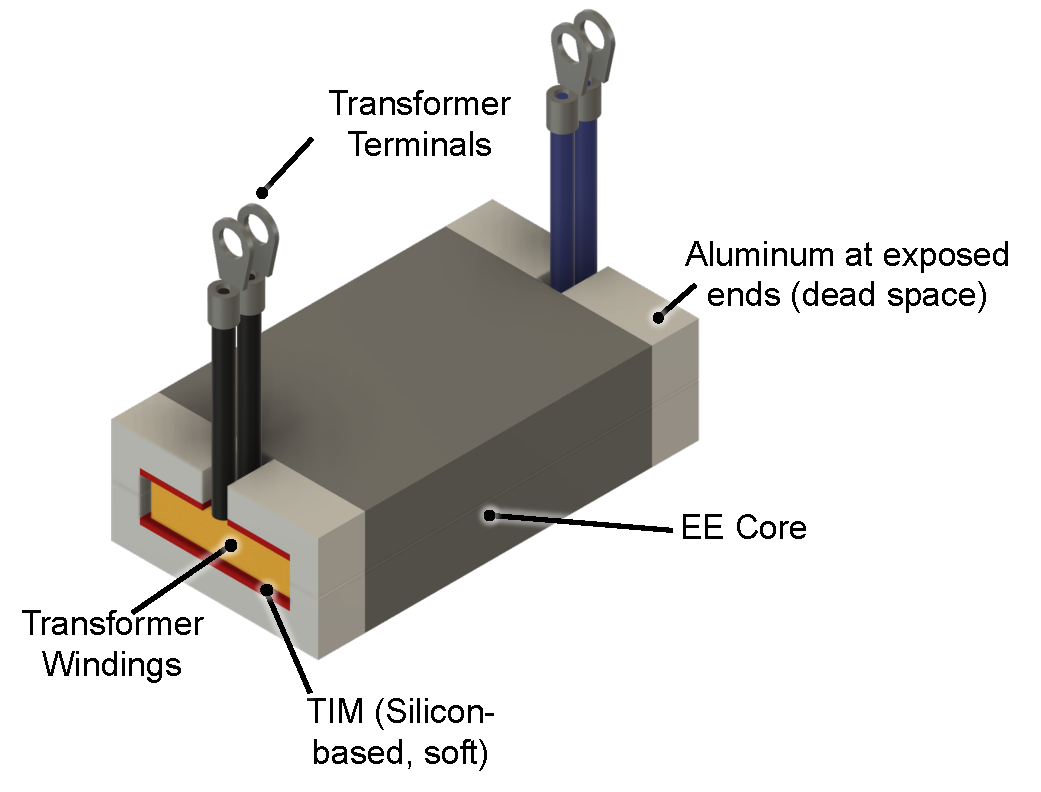
\includegraphics[width=0.6\columnwidth]{figures_intro/concept.pdf}\label{fig:concept_trans}
    }
    \subfloat[]{
    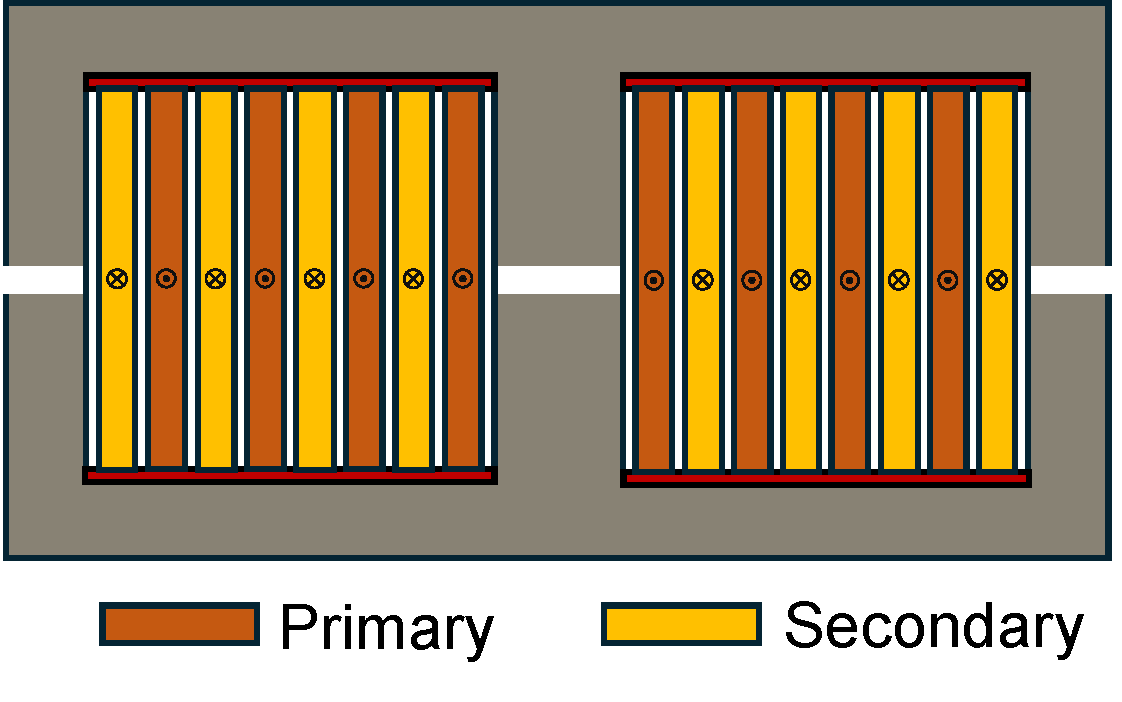
\includegraphics[width=0.4\columnwidth]{figures_intro/concept_cross.pdf}\label{fig:concept_cross}
    }
    \caption{Representative model of an flatwise-wound transformer: (a) mockup of the transformer, and (b) cross-sectional view of the transformer.}
\end{figure}

\section{Objectives of the Study}
\par This study has three main goals. Firstly, this study aims to propose a novel flatwise-wound planar transformer geometry that establishes the internal heat extraction from a restrictive series path to a highly conductive parallel path. Important parameters, such as the AC winding losses, core losses, and magnetizing inductance, are examined to properly optimize the physical dimensions of the transformer. A 1D Thermal Network is also proposed to qualitatively examine the heat extraction mechanism of the proposed flatwise structure. Secondly, this study aims to confirm the feasibility and thermal superiority of the proposed transformer in comprehensive 3D Multi-Physics Finite Element Analysis (FEA). The uniform heat distribution and the elimination of the series thermal bottleneck are confirmed in simulation. Lastly, this study aims to experimentally verify the thermal stability offered by the proposed flatwise design. A continuous full-load operational comparison against its conventional,edgewise-wound counterpart is also performed in this study. The advantage of the proposed configuration is also compared both in simulation and experiment to its conventional counterpart. The concept is proven with a 1-kW, 100V:100 V, 28.5-kHz bidirectional CLLC resonant converter, which is the small-scale counterpart of its high-power 100 kW, 1000V:1000V CLLC for the isolation stage of the SST. 

\section{Significance of the Study}
\par This study is expected to contribute significantly to the existing field of high-power isolation transformers for SST applications. The geometric method presented in this study improves the intrinsic thermal management of the transformer, thereby reducing the dependence on active cooling systems and unlocking higher limits for volumetric power density. Furthermore, while extensive research exists on optimizing the electrical parameters of planar magnetics, studies specifically focusing on the internal thermal path packaging and physical layout optimization are less common. This research directly contributes to bridging the gap between electromagnetic performance and mechanical thermal reliability. Lastly, as a scalability analysis was performed, it provides a lot of insights as to what could be done in future iterations of this work.
\section{Flow of the Paper}
The flow of the paper is structured as follows:
\begin{itemize}
\item \textbf{Chapter 2} presents the motivations behind the selection of the application circuit, which is the bidirectional CLLC resonant converter. It defines the industrial system specifications, the operational modes and adaption to a small-scale study.
\item \textbf{Chapter 3} details the design methodology of the proposed flatwise-wound transformer. It establishes the intrinsic thermal management concept through 1D thermal models, and the analytical equations used to design the transformer.
\item \textbf{Chapter 4} examines the proposed transformer through 3D FEA multi-physics simulations, providing a direct thermal and electrical comparison between the flatwise and conventional edgewise geometries.
\item \textbf{Chapter 5} presents an experimental comparison. A 1 kW proof-of-concept comparison between the proposed flatwise-wound and conventional edgewise-wound structure is evaluated using a representative model with a square window area under continuous operation.
\item \textbf{Chapter 6} presents a conservative, thermal scalability analysis in terms of spatial geometry and operational power. The analysis in Chapter 4 is extended to examine how the thermal benefit of the proposed configuration performs in different spatial profiles and its potential to operate at higher power levels has been examined. 
\item \textbf{Chapter 7} provides the conclusions drawn from the present status of the work and outlines recommendations for future research prospects.
\end{itemize}

\section{About This Work}
This research project is performed in collaboration with ABB Oy and HighQ Power Oy to meet next-generation industrial power conversion demands.

Portions of this study were presented at the \textit{IEEE Applied Power Electronics Conference and Exposition (APEC)}, held in San Antonio, Texas, USA in March 2026. The content included in that presentation focuses primarily on the analytical design and thermo-electromagnetic simulation discussed in Chapter 3 and Chapter 4.

Furthermore, more findings from this work were presented at the \textit{International Conference on Materials and Systems for Sustainability (ICMaSS)} held in Nagoya, Japan in December 2025 and the \textit{IEEE International Power Electronics Conference (IPEC)}, held in Nagasaki, Japan in June 2026. The content of those presentations focuses on the geometric thermal analysis detailed in Chapter 4 and the experimental comparison presented in Chapter 5.


